%%%%%%%%%%%%%%%%%%%%%%%%%%%%%%%%%%%%%%%%%
% Ay 190 - WS2
% Written by Chatarin Wong-u-railertkun
%%%%%%%%%%%%%%%%%%%%%%%%%%%%%%%%%%%%%%%%%

%----------------------------------------------------------------------------------------
%	PACKAGES AND OTHER DOCUMENT CONFIGURATIONS
%----------------------------------------------------------------------------------------

\documentclass[11pt,letterpaper]{article}

% Load some basic packages that are useful to have
% and that should be part of any LaTeX installation.
%

\usepackage{graphicx}     % be able to include figures

\usepackage{xcolor}         % get nice colors

% change default font to Palatino (looks nicer!)
\usepackage[latin1]{inputenc}
\usepackage{mathpazo}
\usepackage[T1]{fontenc}

% load some useful math symbols/fonts
\usepackage{latexsym,amsfonts,amsmath,amssymb}
\usepackage{subcaption}

% comfort package to easily set margins
\usepackage[top=1in, bottom=1in, left=1in, right=1in]{geometry}

% control some spacings
%
% spacing after a paragraph
\setlength{\parskip}{.15cm}
% indentation at the top of a new paragraph
\setlength{\parindent}{0.0cm}

\usepackage{courier}


%----------------------------------------------------------------------------------------
%	TITLE
%----------------------------------------------------------------------------------------

\begin{document}

\begin{center}
\Large
Ay190 -- Worksheet 12 - Solving Poisson Equation \\    %%%%%% DON'T FORGET TO CHANGE THE WORK SHEET NUMBER
Chatarin (Mee) Wong-u-railertkun\\
Date: \today
\end{center}

\section{Determine Columns}

In the data file, we don't know which column represents which quality of the stellar structure, right before the collapse.

\begin{table}[h!]
	\centering
	\begin{tabular}{r || r | r | r | r | r}
		%Table Header
		& Index 0 & Index 1 & Index 2 & Index n-2 & Index n-1 \\
		\hline
		\hline
		% table data
		Col 0 & 1.00000000e+00 & 2.00000000e+00 & 3.00000000e+00 & 1.09700000e+03 & 1.09800000e+03 \\
		Col 1 & 3.97840000e+30 & 8.12410807e+30 & 1.00864534e+31 & 2.17087236e+34 & 2.17092549e+34 \\
		Col 2 & 4.29601329e+06 & 5.46732310e+06 & 5.88378282e+06 & 4.42451097e+13 & 4.44331022e+13 \\
		Col 3 & 7.08374562e+09 & 7.08884898e+09 & 7.09205460e+09 & 2.61019710e+03 & 2.51065707e+03 \\
		Col 4 & 1.19790669e+10 & 1.17625629e+10 & 1.16354022e+10 & 2.11319957e-10 & 1.14387572e-10 \\
		Col 5 & -4.15586982e+06 & -5.28806763e+06 & -5.69046445e+06 & 1.92404912e+03 & 2.21501270e+03 \\
		Col 6 & 0.43135654 & 0.43168572 & 0.43187965 & 0.83966371 & 0.83968791 \\
		Col 7 & 0. & 0. & 0. & 0. & 0. \\
		\hline
	\end{tabular}
	\caption{Showing the first three indices and the last two indices of each column to see the magnitude of values in each column.}
	\label{tab:DataCol}
\end{table}

\begin{figure}[h!]
	\centering
	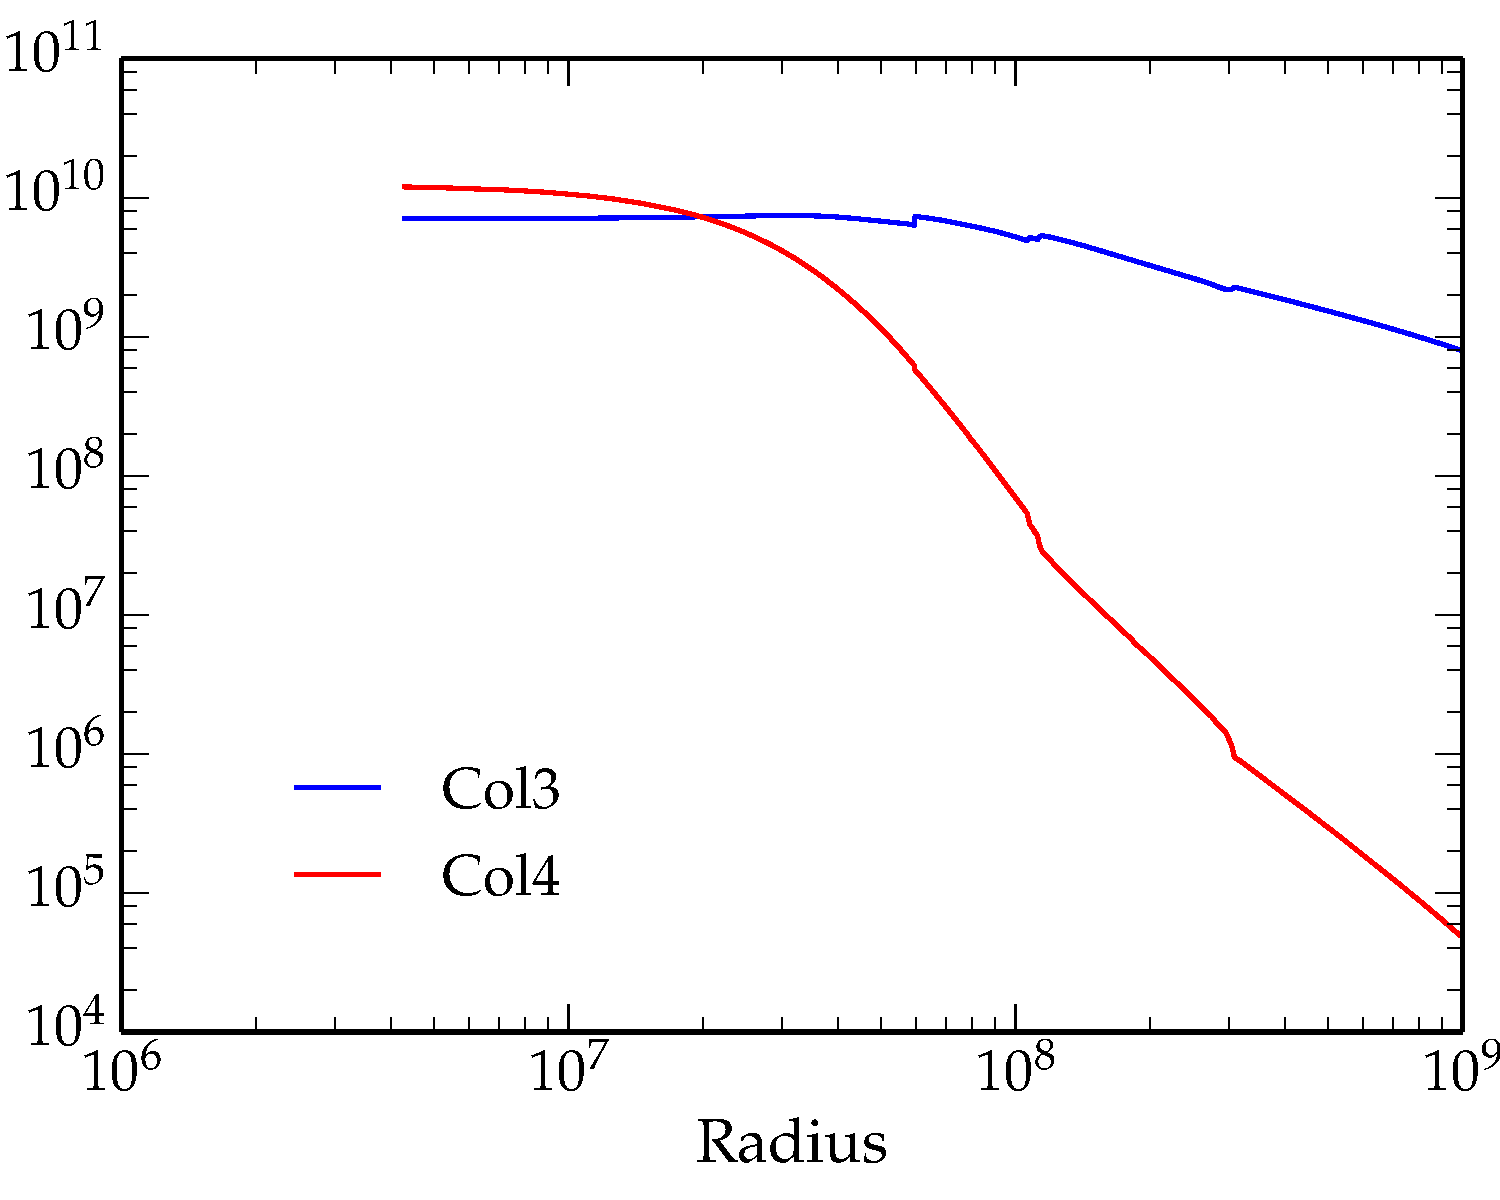
\includegraphics[width=0.5\textwidth]{RhoOrTemp}
	\caption{Compare values of column 3 and 4 vs. radius, to determine which column represents density or temperature.}
	\label{fig:RhoOrTemp}
\end{figure}

Column 0 is just an index, indicating phase of the star. Column 1's dimension suggest that it represents mass. The last entry of column 2 suggests that it represents radius.
Only column 3 and 4 are in the same dimension as expected density. In figure \ref{fig:RhoOrTemp}, we plot those columns against radius. Column 3 occasionally increases, which is impossible for density. Thus, we conclude that column 3 is temperature and column 4 is density.
Column 5 has negative numbers, so we conclude that it represents radial velocity.

\section{Constant Density}

For a sphere with constant density, we can see that our numerical result is similar to the analytical answer. When we compare the absolute error of phi at r=surface, we can see in figure \ref{fig:ConverPlot} the convergence rate.

\begin{figure}[h!]
	\centering
	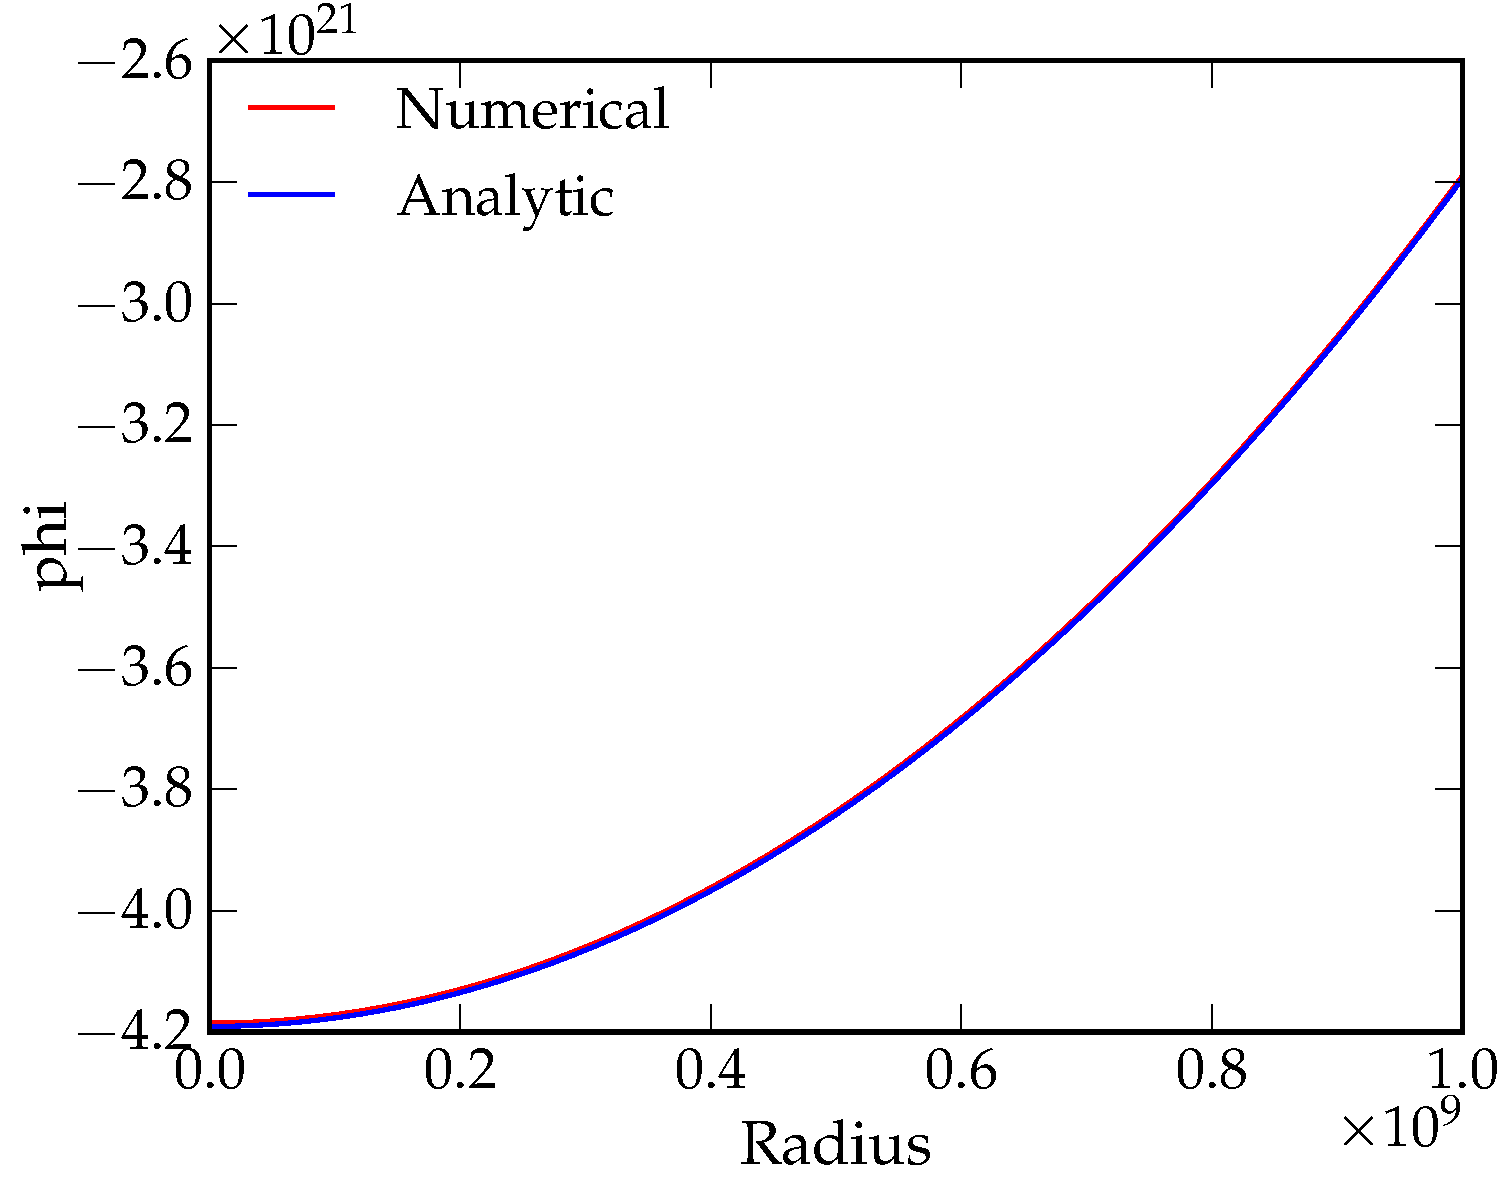
\includegraphics[width=0.5\textwidth]{ConRho}
	\caption{Comparing phi of constant density sphere between the numerical and analytical answer. We can see that both are similar to each other.}
	\label{fig:ConRho}
\end{figure}

\begin{figure}[h!]
	\centering
	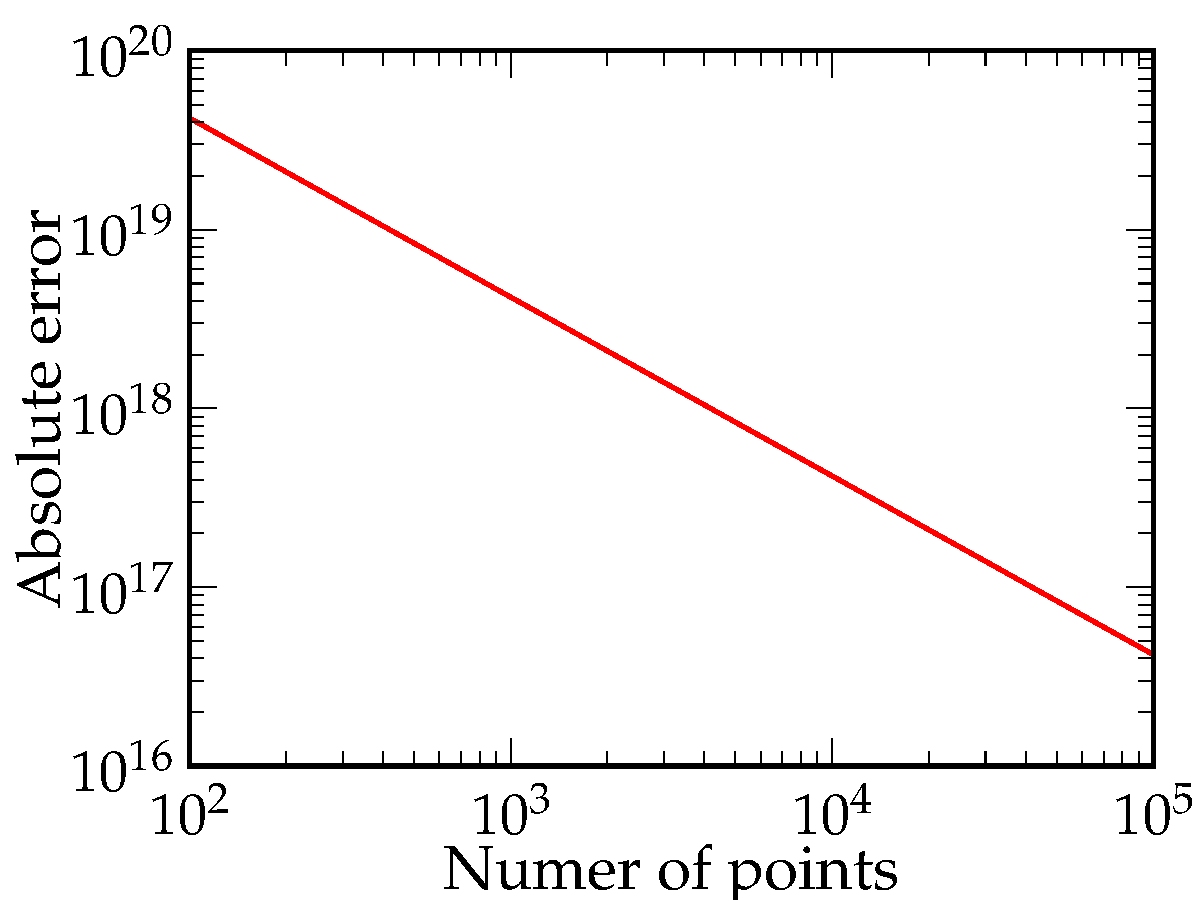
\includegraphics[width=0.5\textwidth]{ConverPlot}
	\caption{Convergent plot of the absolute error of phi at the surface.}
	\label{fig:ConverPlot}
\end{figure}

\newpage
\section{Phi of a star}

Interpolate the density into equilateral grid, then again perform the forward Euler integration.

\begin{figure}[h!]
	\centering
	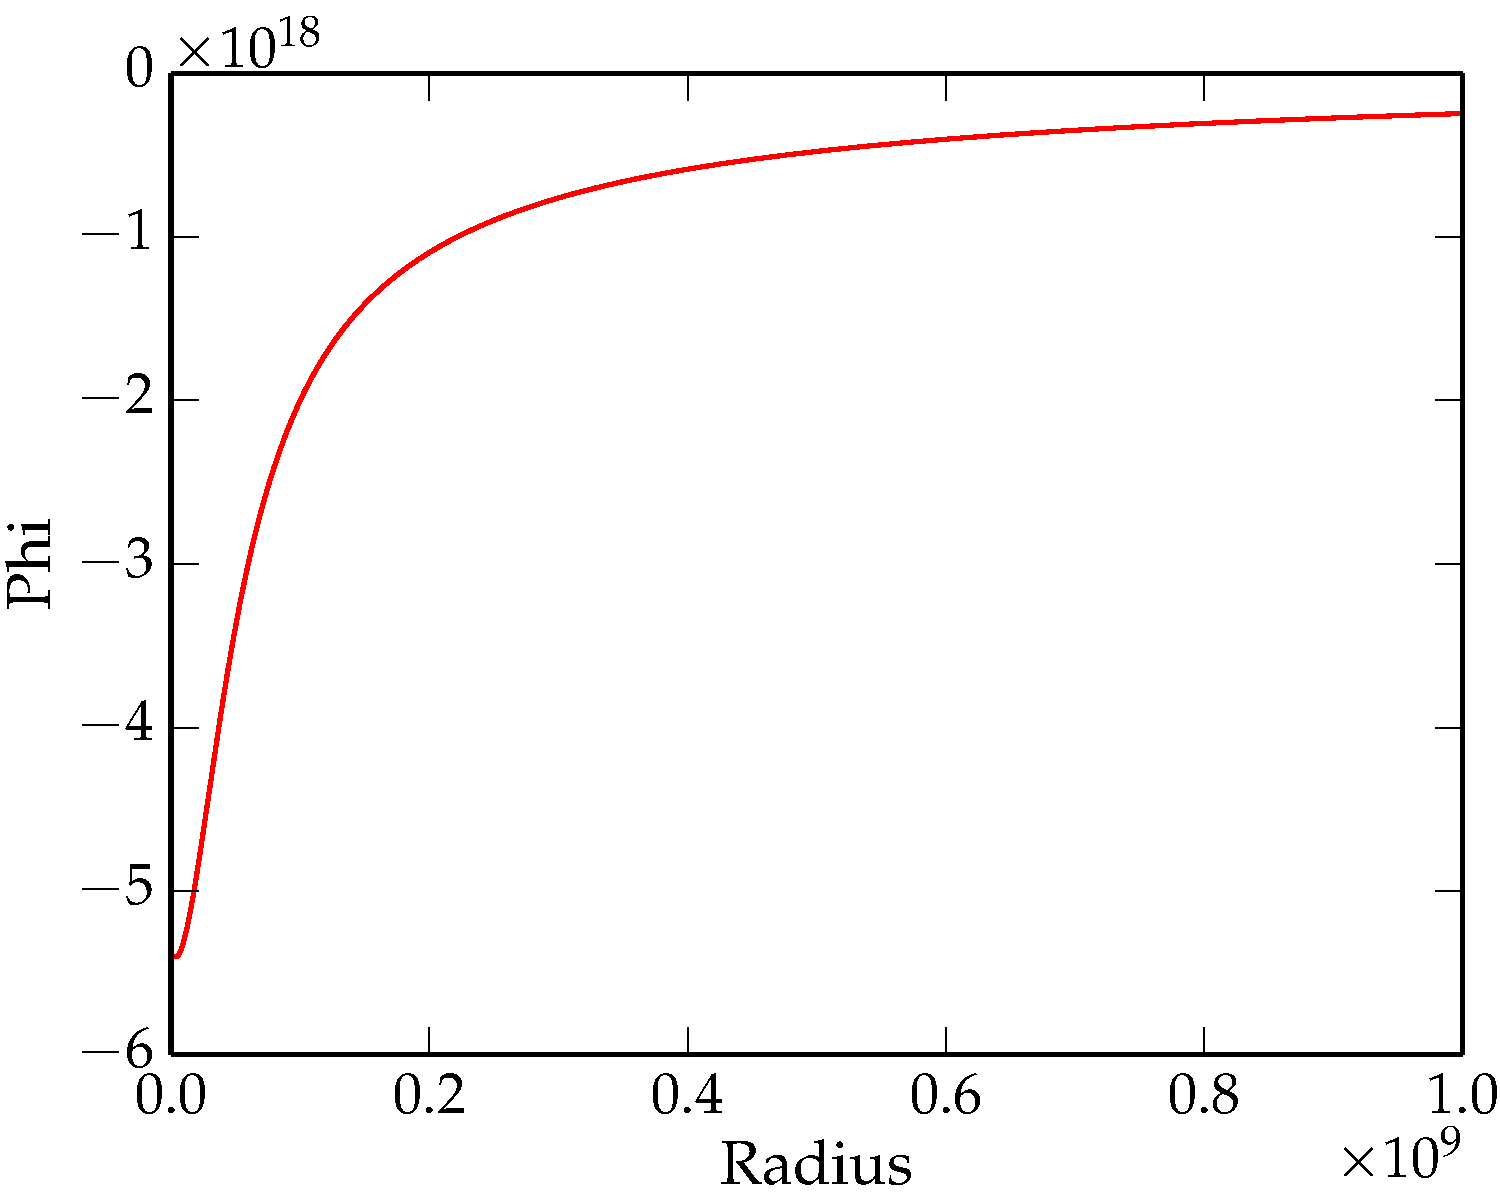
\includegraphics[width=0.5\textwidth]{StarPhi}
	\caption{Phi of the star, based on density from the stellar structure data file.}
	\label{fig:StarPhi}
\end{figure}

	
\end{document}

